%############################# Anhang #################################
\appendix
%\chapter{Mathematischer Anhang}
%\chapter{Programmcodes}

\chapter{Pseudocode}
This appendix chapter helps understanding the algorithm used for the generation of random routes. The complete algorithm
is depicted in Figure~\ref{fig:flowchart_randomRouteGeneration} and the following Algorithm~\ref{alg:appendix:check_single_tour}
is used to check the volume and weight limit of one single tour.
\begin{algorithm}[ht]
    \caption{Check volume and weight limit}
    \label{alg:appendix:check_single_tour}
    \begin{algorithmic}[1]\onehalfspacing
        \Require{Volume limit $V$, Weight limit $Q$, Uniform distribution $\mathcal{U}(a,b)$}
        \Procedure{Feasible}{$\text{Route}\,R,\, \text{Lower Threshold}\,\delta$}
        \State{Get subset of customers $S$ from route $R$}
        \State{$V^* \gets V \cdot \mathcal{U}(\delta,\,1)$} \Comment{Individual bounds for each single route}
        \State{$Q^* \gets Q \cdot \mathcal{U}(\delta,\,1)$}
        \If{$q(S)\le Q^* \, \wedge \, v(S)\le V^*$} \Comment{Check feasibility}
        \State{\textbf{return} true}
        \Else
        \State{\textbf{return} false}
        \EndIf
        \EndProcedure
    \end{algorithmic}
\end{algorithm}

As the following flowchart contains a lot of information and many different symbols the used terms are explained in
the following. The parameters $\mathcal{I}$, $\alpha$, $\beta$, $\gamma$ and $\delta$ were alredady described in
Section~\ref{sec:DataRetrieval}.

\begin{itemize}\singlespacing
    \item $\mathcal{G}$: Set of found routes
    \item $i$: Current instance
    \item $n$: Numbers of customers / Length of route
    \item $n_{max}$: Maximum numbers of customers in instance $i$
    \item $c$: Counter for inner loops finding no tour
    \item $t$: Iteration counter for inner loop (no function!)
    \item $k$: Counter for found tours in the inner loop
    \item $a$: Counter for failed attempts to find a feasible tour
    \item $x$: Counter for breakups
    \item SuccessBool: Boolean, if at least one route was found in inner loop
    \item BreakBool: Boolean for interrupting current instance $i$, when for one customer number $n$ no route could be found
\end{itemize}



\begin{figure}[ht]
    \centering
    \footnotesize
    \begin{tikzpicture}[
            scale = 0.983, transform shape,node distance=7mm and 11mm,
            >=Latex,
            % Styles
            startstop/.style   = {rectangle, draw, align=center, minimum width=22mm, minimum height=6mm},
            process/.style     = {rectangle, draw, align=center, minimum width=30mm, minimum height=6mm},
            decision/.style    = {diamond, draw, aspect=2, inner sep=1pt, align=center, minimum width=40mm,minimum height=20mm},
            io/.style          = {trapezium, trapezium left angle=60, trapezium right angle=120, draw, align=center, minimum height=6mm},
            connector/.style   = {circle, draw, inner sep=1pt},
            line/.style        = {->}
        ]

        % Nodes
        \node[startstop] (start) {Start RRG ($\mathcal{I}$, $\alpha$, $\beta$, $\gamma$, $\delta$)};
        \node[decision, below=of start] (forI) {$i\in\mathcal{I}$ left?};
        \node[process, left= of forI] (nextI) {Next $i$ \&\\ Save $\mathcal{G}$};
        \node[process, below=of forI] (initI) {$\mathcal{G}\gets\emptyset$\\$n_{\max}\gets \mathrm{MaxCustomers}(i)$\\BreakBool$\gets$False};
        \node[decision, below=5mm of initI] (forN) {$n=2\ \to\ n_{\max}$ left?};
        \node[decision, below=of forN] (exitOuter) {BreakBool?};
        \node[decision, right=of exitOuter] (breakDec) {$c \geq n \cdot \alpha$?};
        \node[startstop] at ($(breakDec.north |- forI.east)$) (end) {End RRG};
        \node[decision, below=of exitOuter] (forAlpha) {$t=1\ \to\ n\cdot\alpha$ left?};
        \node[decision, below=of forAlpha] (whileK) {While\\$k<\gamma$?};
        \node[decision, below=12 mm of whileK] (dup) {$R\in\mathcal{G}$?};
        % \node[process, bel=of dup] (drawThresh) {$Q^*\gets Q\cdot \mathcal{U}_\delta^1$\\$V^*\gets V\cdot \mathcal{U}_\delta^1$};
        \node[decision, right=of dup] (feasible) {Feasible($R$, $\delta$)?\\(See Alg.~\ref{alg:appendix:check_single_tour})};
        \node[process, above=10mm of feasible] (accept) {$\mathcal{G}\gets \mathcal{G}\cup\{R\}$\\SuccessBool$\gets$True};
        \node[decision, below= of feasible] (attemptCond) {$a\ge \beta$?};
        \node[process] at ($(dup.south |- attemptCond.west)$) (incX) {$x\gets x+1$};
        \node[process, left=of dup] (incC) {$c\gets c+1$};
        \node[decision] at ($(incC.south |- incX.west)$)  (breakCond) {$x\ge \gamma$ \& \\$\overline{\text{SuccessBool}}$?};
        \node[process] at ($(breakDec.north |- forN.east)$) (trueExit) {BreakBool$\gets$True};

        % Edges
        \draw[line] (start) -- (forI);
        \draw[line] (forI) -- node[pos=0.5, right]{yes}(initI);
        \draw[line] (forI) -- node[pos=0.5, above]{no}(end);
        \draw[line] (initI) -- (forN);
        \draw[line] (nextI.east)-- (forI.west);
        \draw[line] (forAlpha.east) -| node[pos = 0.25,above]{no}(breakDec.south);
        \draw[line] (breakDec.west) -- node[pos = 0.5,above]{no}($(breakDec.west)-(5mm,0)$) |- (forN.east);
        \draw[line] (breakDec) -- node[pos = 0.5,right]{yes}(trueExit);
        \draw[line] (trueExit) -- (forN);
        \draw[line] (whileK.west) -- ($(whileK.west)-(10mm,0)$) coordinate (bend) node[pos = 0.5,above]{no} |- (forAlpha.west);

        \draw[line] (forN.south) --  node[pos=0.5, right]{yes}(exitOuter.north);
        \draw[line] (forN.west) -|  node[pos=0.25, above]{no}(nextI.south);
        \draw[line] (exitOuter.west) -| node[pos=0.25, above]{yes} (nextI.south);

        \draw[line] (exitOuter) -- node[pos=0.5, right, align=left]{no\\$c \gets 0$} (forAlpha);

        \draw[line] (forAlpha) -- node[pos=0.5, right, align=left]{$k,a,x\gets 0$\\ SuccessBool$\gets$False} (whileK);
        \draw[line] (whileK) --node[pos=0.5, right, align=left]{yes \\ $R\gets \mathrm{RandomTour}(i,n)$} (dup);
        \draw[line] (dup) -- node[pos=0.5, below]{no}(feasible);
        \draw[line] (dup) -- node[pos=0.5, right]{yes}(incX);
        \draw[line] (incX) -- (breakCond);
        %\draw[line] (breakCond) -- node[pos=0.25, below right]{no}(whileK);
        \draw[line] (breakCond) |- node[pos=0.5, left]{no}($(incX.south)-(0,10mm)$) -| ($(attemptCond.east)+(10mm,0)$) coordinate (bend)|- (whileK);
        \draw[line] (breakCond) -- node[pos=0.5, left]{yes} (incC);
        \draw[line] (incC) |- (forAlpha);

        \draw[line] (feasible) -- node[pos=0.5, left]{yes}(accept);
        \draw[line] (feasible) -- node[pos=0.5, right, align=left]{$a \gets 0$ \\ $k\gets k+1$}(accept);
        \draw[line] (accept.north) |- (whileK.east);

        \draw[line] (feasible) --node[pos=0.5, right, align=left]{no\\$a\gets a+1$} (attemptCond);
        \draw[line] (attemptCond) --node[pos=0.5, above, align=center]{yes\\$a\gets 0$} (incX);
        \draw[line] (attemptCond) -- ($(attemptCond.east)+(10mm,0)$) coordinate (bend) node[pos = 0.5,above]{no} |- (whileK);

        % Labels for the for-loops (optional, visual clarity)
        \node[above left=0mm and -3mm of forI] {\footnotesize For each $i\in\mathcal{I}$};
        \node[above left=0mm and -3mm of forN] {\footnotesize For $n=2,\dots,n_{\max}$};
        \node[above left=0mm and -1mm of forAlpha] {\footnotesize For $t=1,\dots,n\alpha$};

    \end{tikzpicture}
    \caption{Flowchart for Random Routes Generation (RRG).}
    \label{fig:flowchart_randomRouteGeneration}
\end{figure}

\chapter{Feature Selection}
\label{app:feature_selection}

\chapter{Parking Lot}
\label{app:trash}
With a subset from krebs the following datasets were created!
\begin{table}[ht]
    \centering
    \begin{tabular}{c c cc c c c}
        \hline
        \makecell{Multiplier $\alpha$} & \makecell{Attempts                          \\ limit $\beta$} & \makecell{Success \\threshold $\gamma$} & Routes & Balance& \gls{MCC}-Score & F1-Score \\
        \hline
        1                              & 1                  & 1 & 7616  & 60/40 &  & \\
        1                              & 1                  & 2 & 15948 & 60/40 &  & \\
        1                              & 1                  & 3 & 24573 & 60/40 &  & \\
        1                              & 2                  & 1 & 8325  & 60/40 &  & \\
        1                              & 2                  & 2 & 17217 & 60/40 &  & \\
        1                              & 2                  & 3 & 26467 & 60/40 &  & \\
        1                              & 3                  & 1 & 8683  & 60/40 &  & \\
        1                              & 3                  & 2 & 18041 & 60/40 &  & \\
        1                              & 3                  & 3 & 27535 & 60/40 &  & \\
        \hline
    \end{tabular}
    \caption[Created instances for different parameter combinations $(\alpha, \beta, \gamma)$ for \krebsADataSetText dataset.]{Created instances for different parameter combinations $(\alpha, \beta, \gamma)$ for \krebsADataSetText dataset.
        The values in the balance column stand for the share of positive and netative labels in the sample population.}
    \label{tab:created_instances_xyz_krebs}
\end{table}



\begin{table}[ht]
    \centering
    \begin{tabular}{c c c c c c}
        \toprule
        Model                          & Name     & \gls{MCC}-Score & \gls{AUROC} & F1-Score & Accuracy \\
        \midrule
        \multirow{3}{*}{\gls{LR}}      & Complete & 0.6             & 0.9         & 0.87     & 0.95     \\
                                       & Trimmed  & 0.6             & 0.9         & 0.87     & 0.95     \\
                                       & Shrinked & 0.6             & 0.9         & 0.87     & 0.95     \\
        \midrule
        \multirow{3}{*}{Decision Tree} & Complete & 0.6             & 0.9         & 0.87     & 0.95     \\
                                       & Trimmed  & 0.6             & 0.9         & 0.87     & 0.95     \\
                                       & Shrinked & 0.6             & 0.9         & 0.87     & 0.95     \\
        \midrule
        \multirow{3}{*}{\gls{FFNN}}    & Complete & 0.6             & 0.9         & 0.87     & 0.95     \\
                                       & Trimmed  & 0.6             & 0.9         & 0.87     & 0.95     \\
                                       & Shrinked & 0.6             & 0.9         & 0.87     & 0.95     \\
        \bottomrule
    \end{tabular}
    \caption{Results}
    \label{tab:dataset_model_selection_saveStrategy}
\end{table}

\begin{table}[ht]
    \centering
    \begin{tabular}{c c c c c c}
        \toprule
        Model                           & Name       & \gls{MCC}-Score & \gls{AUROC} & F1-Score & Accuracy \\
        \midrule
        \multirow{13}{*}{\gls{LR}}      & RD-2-20-20 & 0.6             & 0.9         & 0.87     & 0.95     \\
                                        & RD-2-20-30 & 0.6             & 0.9         & 0.87     & 0.95     \\
                                        & RD-2-30-20 & 0.6             & 0.9         & 0.87     & 0.95     \\
                                        & RD-2-30-30 & 0.6             & 0.9         & 0.87     & 0.95     \\
                                        & RD-3-20-20 & 0.6             & 0.9         & 0.87     & 0.95     \\
                                        & RD-3-20-30 & 0.6             & 0.9         & 0.87     & 0.95     \\
                                        & RD-3-30-20 & 0.6             & 0.9         & 0.87     & 0.95     \\
                                        & RD-3-30-30 & 0.6             & 0.9         & 0.87     & 0.95     \\
                                        & RD-4-20-20 & 0.6             & 0.9         & 0.87     & 0.95     \\
                                        & RD-4-20-30 & 0.6             & 0.9         & 0.87     & 0.95     \\
                                        & RD-4-30-20 & 0.6             & 0.9         & 0.87     & 0.95     \\
                                        & RD-4-30-30 & 0.6             & 0.9         & 0.87     & 0.95     \\
                                        & RD-5-40-40 & 0.6             & 0.9         & 0.87     & 0.95     \\
        \midrule
        \multirow{13}{*}{Decision Tree} & RD-2-20-20 & 0.6             & 0.9         & 0.87     & 0.95     \\
                                        & RD-2-20-30 & 0.6             & 0.9         & 0.87     & 0.95     \\
                                        & RD-2-30-20 & 0.6             & 0.9         & 0.87     & 0.95     \\
                                        & RD-2-30-30 & 0.6             & 0.9         & 0.87     & 0.95     \\
                                        & RD-3-20-20 & 0.6             & 0.9         & 0.87     & 0.95     \\
                                        & RD-3-20-30 & 0.6             & 0.9         & 0.87     & 0.95     \\
                                        & RD-3-30-20 & 0.6             & 0.9         & 0.87     & 0.95     \\
                                        & RD-3-30-30 & 0.6             & 0.9         & 0.87     & 0.95     \\
                                        & RD-4-20-20 & 0.6             & 0.9         & 0.87     & 0.95     \\
                                        & RD-4-20-30 & 0.6             & 0.9         & 0.87     & 0.95     \\
                                        & RD-4-30-20 & 0.6             & 0.9         & 0.87     & 0.95     \\
                                        & RD-4-30-30 & 0.6             & 0.9         & 0.87     & 0.95     \\
                                        & RD-5-40-40 & 0.6             & 0.9         & 0.87     & 0.95     \\
        \midrule
        \multirow{13}{*}{\gls{FFNN}}    & RD-2-20-20 & 0.6             & 0.9         & 0.87     & 0.95     \\
                                        & RD-2-20-30 & 0.6             & 0.9         & 0.87     & 0.95     \\
                                        & RD-2-30-20 & 0.6             & 0.9         & 0.87     & 0.95     \\
                                        & RD-2-30-30 & 0.6             & 0.9         & 0.87     & 0.95     \\
                                        & RD-3-20-20 & 0.6             & 0.9         & 0.87     & 0.95     \\
                                        & RD-3-20-30 & 0.6             & 0.9         & 0.87     & 0.95     \\
                                        & RD-3-30-20 & 0.6             & 0.9         & 0.87     & 0.95     \\
                                        & RD-3-30-30 & 0.6             & 0.9         & 0.87     & 0.95     \\
                                        & RD-4-20-20 & 0.6             & 0.9         & 0.87     & 0.95     \\
                                        & RD-4-20-30 & 0.6             & 0.9         & 0.87     & 0.95     \\
                                        & RD-4-30-20 & 0.6             & 0.9         & 0.87     & 0.95     \\
                                        & RD-4-30-30 & 0.6             & 0.9         & 0.87     & 0.95     \\
                                        & RD-5-40-40 & 0.6             & 0.9         & 0.87     & 0.95     \\
        \bottomrule
    \end{tabular}
    \caption{Results}
    \label{tab:dataset_model_selection_randomStrategy}
\end{table}

\chapter{Parameterstudy}

\begin{figure}[ht]
    \centering
    \begin{tikzpicture}[node distance=0mm and 0mm]
        \node[anchor=south, inner sep=0] (A) at (0,0)
        {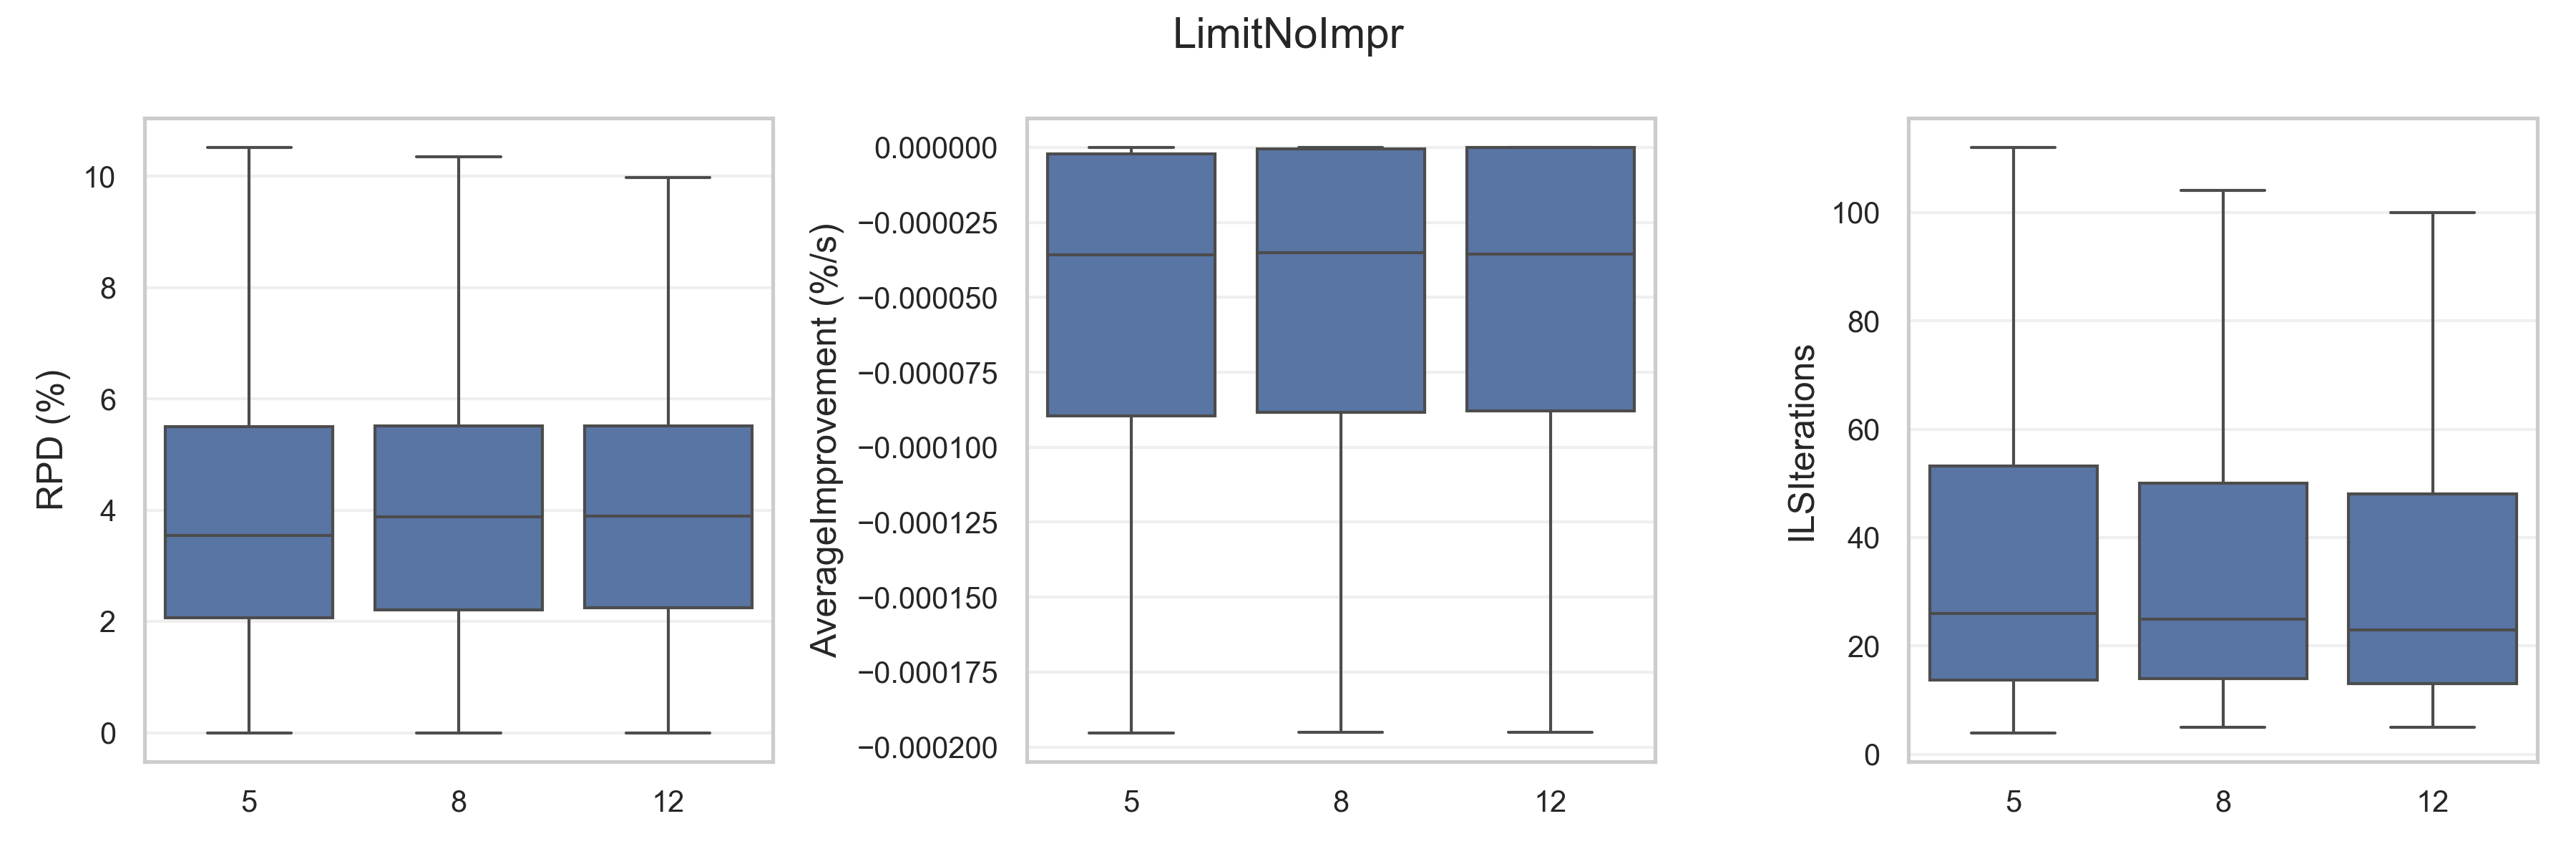
\includegraphics[width=0.95\textwidth]{pictures/parameter_study/LimitNoImpr_base_parameter_study.png}};
        \node[anchor=north, below=of A,inner sep=0] (B)
        {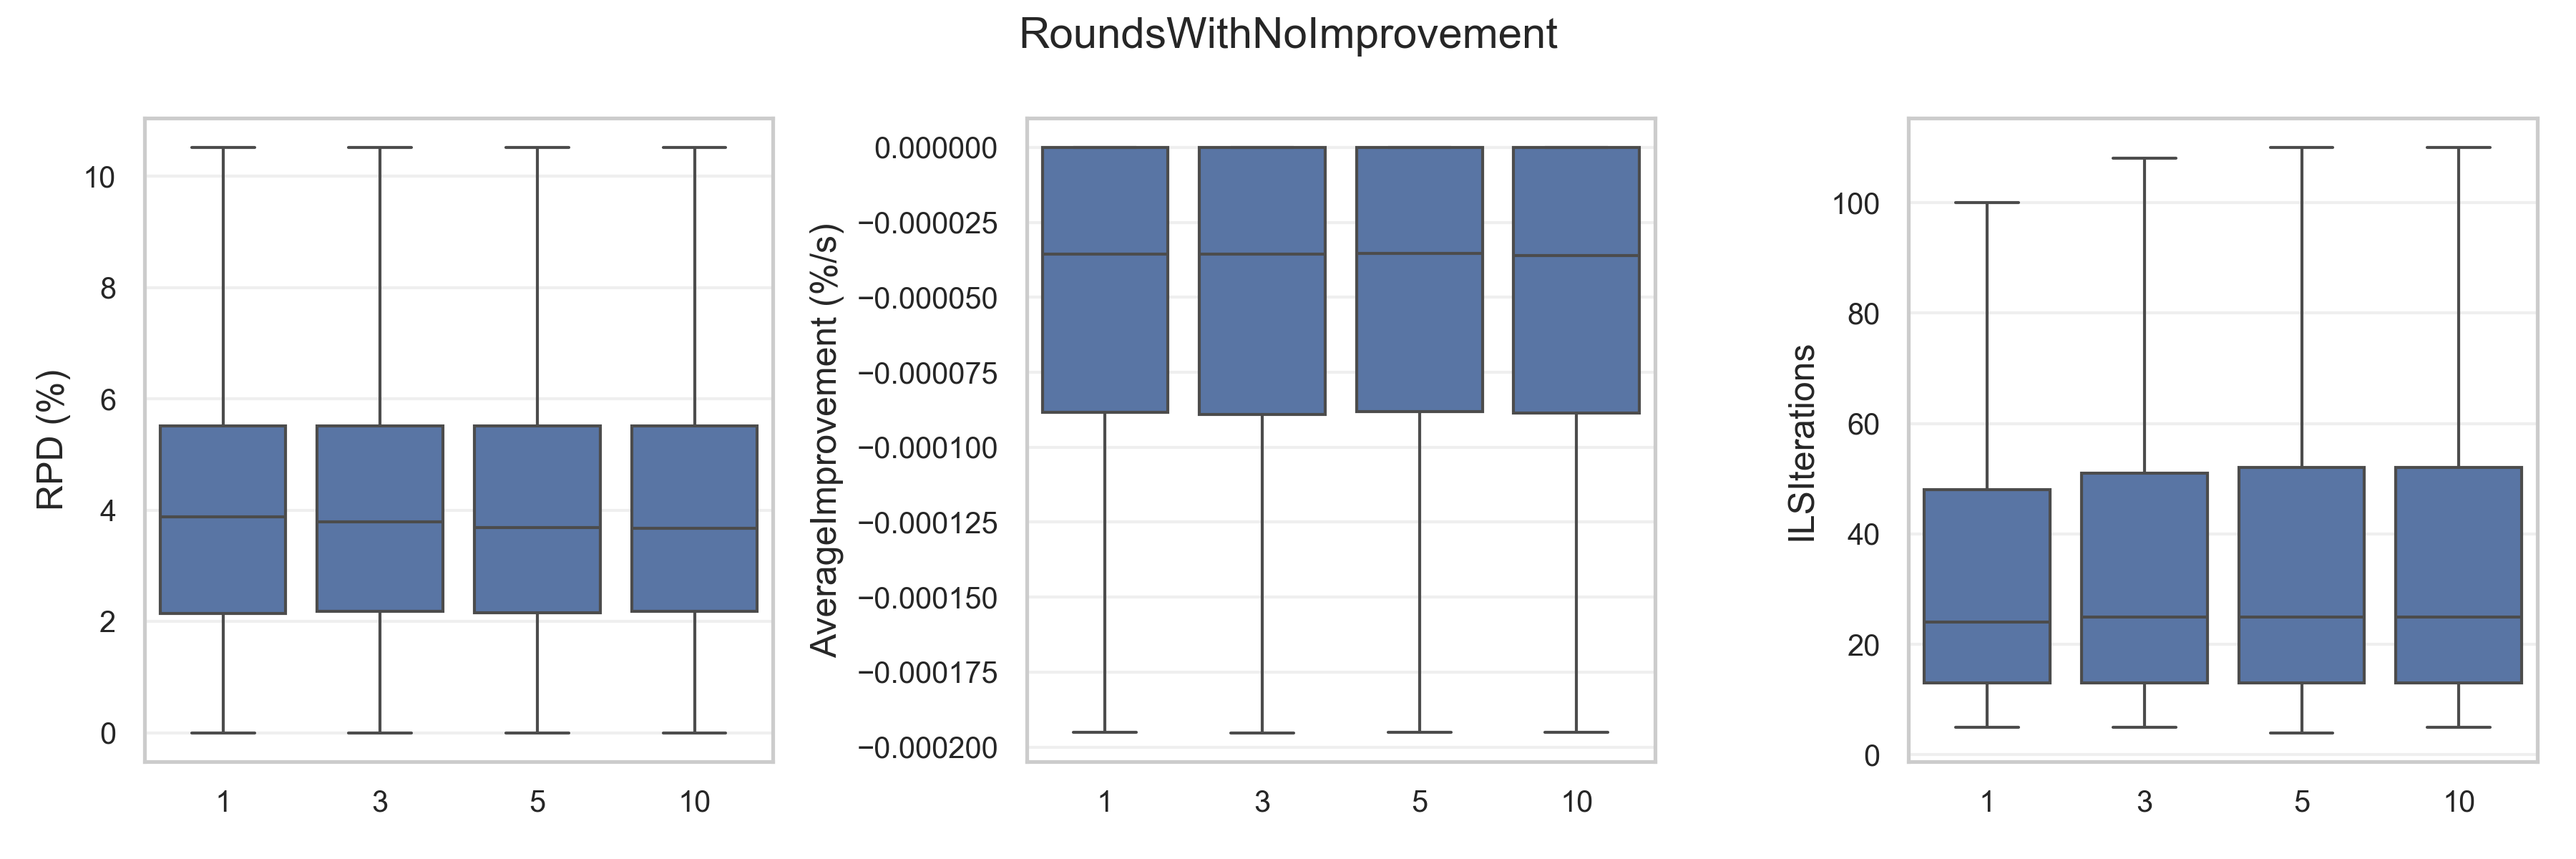
\includegraphics[width=0.96\textwidth]{pictures/parameter_study/RoundsWithNoImprovement_base_parameter_study.png}};
    \end{tikzpicture}
    \caption{Results of the parameterstudy for NoClassifier variant and different levels for the the maximum rounds and iterations without improvement.}
    \label{fig:aggregated_base_parameter_study_appendix}
\end{figure}